%%%%%%%%%%%%%%%%%%%%%%%%%%%%%%%%%%%%%%%%%%%%%%%%%%%%%%%%%%%%%%%%%%%%%%%%
% Escuela Politécnica Superior de la Universidad de Alicante
% Realizado por: Jose Manuel Requena Plens
% Contacto: info@jmrplens.com / Telegram:@jmrplens
%%%%%%%%%%%%%%%%%%%%%%%%%%%%%%%%%%%%%%%%%%%%%%%%%%%%%%%%%%%%%%%%%%%%%%%%

\definecolor{mycolor1}{rgb}{0.00000,0.44700,0.74100}%
%
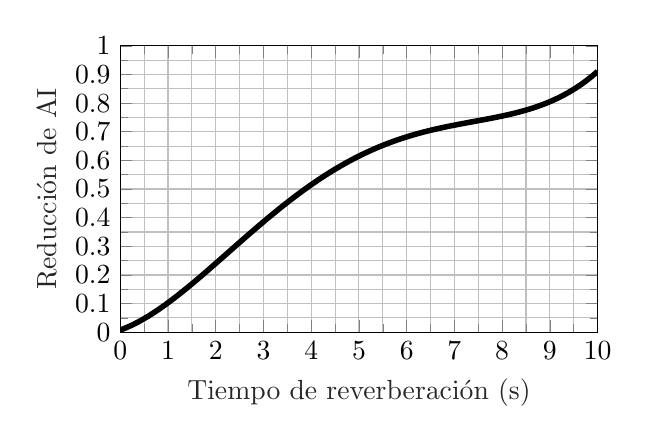
\begin{tikzpicture}

\begin{axis}[%
width=0.5\textwidth,
height=0.3\textwidth,
at={(0\textwidth,0\textwidth)},
scale only axis,
xmin=0,
xmax=10,
xlabel style={font=\color{white!15!black}},
xlabel={Tiempo de reverberación (s)},
xtick distance=1,
minor x tick num= 1,
minor y tick num= 1,
ymin=0,
ymax=1,
ytick distance=0.1,
grid=both,
ylabel style={font=\color{white!15!black}},
ylabel={Reducción de AI},
axis background/.style={fill=white},
legend style={legend cell align=left, align=left, draw=white!15!black}
]

\addplot[color=black,line width=2.0pt,domain=0:10, samples=85]{0.0004264*x^4 -0.008245*x^3 + 0.04282*x^2 + 0.06021*x + 0.007629};
\end{axis}
\end{tikzpicture}%